
\documentclass[usenames,dvipsnames]{beamer}
\mode<presentation>{\usetheme{Warsaw}}
\usepackage{textpos} %package for text positioning

%%%%%%%%%%%%%%%%%%%%%%%%%%%%%%%%%%%%%%%%%%%%%%%%%%%%%%%%%%%%%%%%%%%%%%%%%%%%%%%%%%%%
%Normal Math Packages
\usepackage{amsmath}
\usepackage{amsfonts}
\usepackage{enumerate}
\usepackage{amsmath}
\usepackage{mathtools}
\usepackage{tikz-cd}
\usepackage{ragged2e}
\usepackage{mathrsfs}
\usepackage{xcolor}
\usepackage{soul}
%%%%%%%%%%%%%%%%%%%%%%%%%%%%%%%%%%%%%%%%%%%%%%%%%%%%%%%%%%%%%%%%%%%%%%%%%%%%%%%%%%%%

%%%%%%%%%%%%%%%%%%%%%%%%%%%%%%%%%%%%%%%%%%%%%%%%%%%%%%%%%%%%%%%%%%%%%%%%%%%%%%%%%%%%
%Created Commands
\theoremstyle{definition}
\newtheorem*{remark}{Remark}
\newtheorem*{question}{Question}
\newtheorem*{answer}{Answer}
\newtheorem*{goal}{Goal}
\newtheorem*{conjecture}{Conjecture}
%\newtheorem*{definition}{Definition}
%\newtheorem*{definitions}{Definitions}

\theoremstyle{theorem}
\newtheorem*{proposition}{Proposition}
\newtheorem*{axiom}{Axiom}

\newcommand{\R}{\mathbb{R}}
\newcommand{\Q}{\mathbb{Q}}
\newcommand{\F}{\mathbb{F}}
\newcommand{\A}{\mathcal{A}}
\newcommand{\N}{\mathbb{N}}
\newcommand{\C}{\mathbb{C}}
\newcommand{\opO}{\mathcal{O}}
\newcommand{\states}{\mathcal{S}}
\newcommand{\position}{\boldsymbol{\gamma}}
\newcommand{\velocity}{\boldsymbol{\dot{\gamma}}}
%%%%%%%%%%%%%%%%%%%%%%%%%%%%%%%%%%%%%%%%%%%%%%%%%%%%%%%%%%%%%%%%%%%%%%%%%%%%%%%%%%%%

%%%%%%%%%%%%%%%%%%%%%%%%%%%%%%%%%%%%%%%%%%%%%%%%%%%%%%%%%%%%%%%%%%%%%%%%%%%%%%%%%%%%
%Pseudocode
\usepackage{algorithm}
\usepackage[noend]{algpseudocode}
%%%%%%%%%%%%%%%%%%%%%%%%%%%%%%%%%%%%%%%%%%%%%%%%%%%%%%%%%%%%%%%%%%%%%%%%%%%%%%%%%%%%


%%%%%%%%%%%%%%%%%%%%%%%%%%%%%%%%%%%%%%%%%%%%%%%%%%%%%%%%%%%%%%%%%%%%%%%%%%%%%%%%%%%%
%Remove buttons
\setbeamertemplate{navigation symbols}{}

%Stuff to make things look good
% Color modification
\setbeamercolor{structure}{fg=green!30!black}% to modify  immediately all palettes
\setbeamercolor{title}{fg=white}
\setbeamercolor{title in head/foot}{fg=yellow}

%Size Modification
\setbeamerfont{frametitle}{size=\Large}

% position the logo
\addtobeamertemplate{frametitle}{}{%
\begin{textblock*}{1cm}(.985\textwidth,-1.25cm)

\includegraphics[height=1cm,width=1cm,keepaspectratio]{csu.png}
\end{textblock*}}

% Text Positioning
\usepackage[absolute,overlay]{textpos}
%%%%%%%%%%%%%%%%%%%%%%%%%%%%%%%%%%%%%%%%%%%%%%%%%%%%%%%%%%%%%%%%%%%%%%%%%%%%%%%%%%%%

%Font
%\fontfamily{cmr}\selectfont
\usefonttheme{serif}

%Colors and stuf
\usepackage{color, soul, xcolor} % Colored text and highlighting, respectively
\usepackage{tikz-cd} % For commutative diagrams

%% preamble
\title{Harmonic Maps and Gradient Flow}
\subtitle{Math 546 Project}
\author{Colin Roberts}

\begin{document}

%%Title Frame
{
\setbeamertemplate{headline}{}
\addtobeamertemplate{frametitle}{\vspace*{-0.9\baselineskip}}{}
\begin{frame}
\titlepage
\end{frame}
}

%Table of contents slide

%\AtBeginSection[]
%{
%	\begin{frame}{Table of Contents}
%		\tableofcontents[currentsection]
%	\end{frame}
%}

%%%%%%%%%%%%%%%%%%%%%%%%%%%%%%%%%%%%%%%%%%%%%%%%%%%%%%%%%%%%%%%%%%%%%%%%%%%%%%%
%%%%%%%%%%%%%%%%%%%%%%%%%%%%%%%%%%%%%%%%%%%%%%%%%%%%%%%%%%%%%%%%%%%%%%%%%%%%%%%

\section{Overview}
    
    \subsection{Motivation}
    
        \begin{frame}{The Story}
            \begin{enumerate}
                \item Optimization problems are abundant and important.
                \pause
                \item One specific example is found in optimizing energy of elastic materials.
                \pause
                \item There is an analogy with heat flow that allows us to find these optimizing states for general optimization problems.
            \end{enumerate}
        \end{frame}
        
        \begin{frame}{The Motivating Questions}
            \begin{question}
            What is the elastic energy functional?
            \end{question}
            
            \begin{question}
            What are the functions that optimize this energy?
            \end{question}
            
            \begin{question}
            Is there a method or algorithm to search for an optimizer by starting at any point in our space?
            \end{question}
        \end{frame}
        
        \begin{frame}{Applications}
            \begin{center}
                \textbf{\underline{Real World Applications}}
            \end{center}
            \begin{itemize}
                \item Building 3D (printing) structures.
                \item Machine learning.
                \item Smoothing noisy data.
            \end{itemize}
            \begin{center}
                \vspace*{.5cm}
                \pause
                \textbf{\underline{Mathematical Applications}}
            \end{center}
            \begin{itemize}
                \item Framework for optimization problems.
                \item Existence of minimal mappings.
                \item Solution to the Poincar\'e conjecture.
            \end{itemize}
        \end{frame}
        
        \begin{frame}{Aside}
            \begin{conjecture}
                Every simply connected, closed 3-manifold is homeomorphic to the 3-sphere.
            \end{conjecture}
            \pause
            In other words,
            \begin{itemize}
                \item Place a closed loop on a 3-dimensional manifold.
                \pause
                \item Contract the loop over time.
                \pause
                \item Does this process limit to a point?
            \end{itemize}
            \pause
            \begin{remark}
            Keep this process in mind!
            \end{remark}
        \end{frame}
        
        \begin{frame}{Aside}
            \begin{figure}[H]
            \centering
            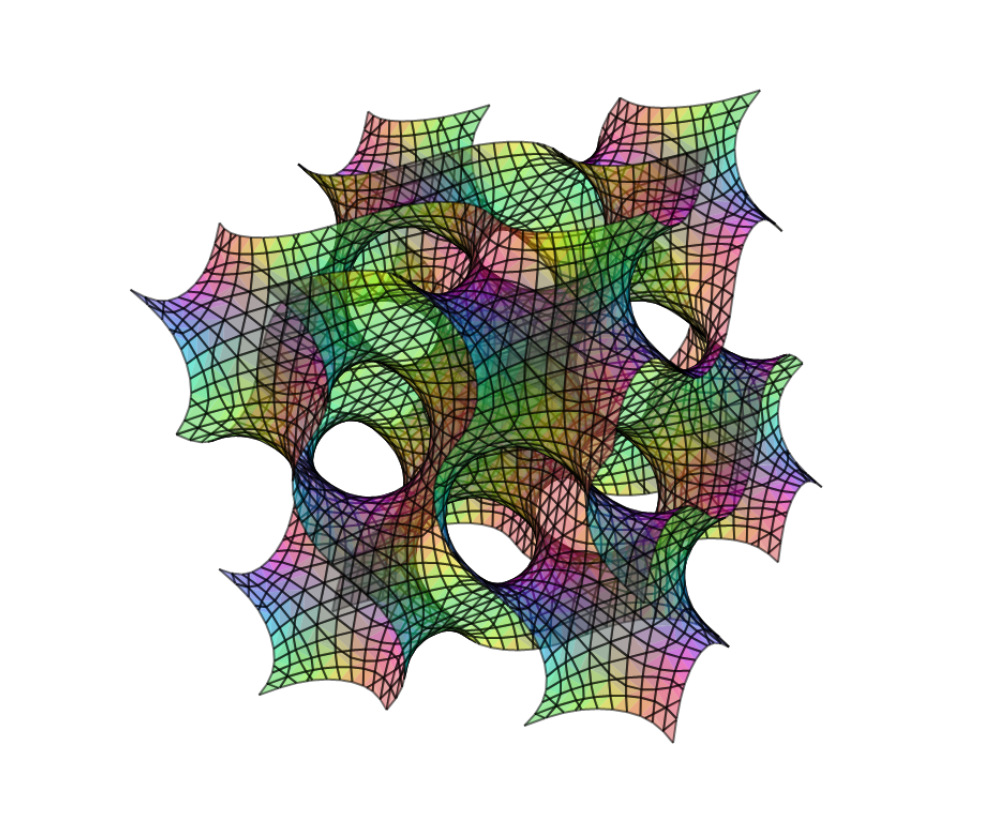
\includegraphics[width=.6\textwidth]{images/gyroid_fixed.png}
            \caption{The Gyroid minimimal surface.}
            \end{figure}
        \end{frame}
        
        \begin{frame}{The Motivating Problems}
            \begin{itemize}
            \begin{minipage}{0.55\linewidth}
                \item[] \textbf{\underline{Geometry}}
                \item Geodesics
                \item Minimal Submanifolds
                \item Gradient Flow
            \end{minipage}
            \begin{minipage}{0.4\linewidth}
                \item[] \textbf{\underline{Physics}}
                \item Free Particles
                \item Elastic Materials
                \item Heat Flow
            \end{minipage}
            \end{itemize}
        \end{frame}
        
    \subsection{Problem Setting}

        \begin{frame}{Geodesics}
            \emph{Geodesics} $\gamma$ are curves on a manifold $M$ satisfying a few equivalent definitions.
            \begin{itemize}
                \item $\gamma$ is the shortest path between two points on $M$.
                \item $\gamma$ is the least curved path between two points on $M$.
                \item $\gamma$ is a trajectory of a free particle on $M$.
                \item $\gamma$ minimizes the Dirichlet energy.
            \end{itemize}
        \end{frame}
        
            \begin{frame}{Geodesics}
            \emph{Geodesics} $\gamma$ are curves on a manifold $M$ satisfying a few equivalent definitions.
            \begin{itemize}
                \item $\gamma$ is the shortest path between two points on $M$.
                \item $\gamma$ is the least curved path between two points on $M$.
                \item $\gamma$ is a trajectory of a free particle on $M$.
                \item \colorbox<1>{yellow}{$\gamma$ minimizes the Dirichlet energy.}
            \end{itemize}
        \end{frame}
        
        \begin{frame}{Minimal Surfaces}
             Fix a closed curve $\Gamma$ and a surface $\Sigma$ with $\partial \Sigma = \Gamma$. The following are equivalent definitions of a \emph{minimal surface}.
            \begin{itemize}
                \item $\Sigma$ minimizes the area functional.
                \item $\Sigma$ has zero mean curvature.
                \item $\Sigma$ is a critical point of the mean curvature flow.
                \item $\Sigma$ minimizes the Dirichlet energy.
            \end{itemize}
        \end{frame}
        
        \begin{frame}{Minimal Surfaces}
             Fix a closed curve $\Gamma$ on $M$ and a surface $\Sigma$ with $\partial \Sigma = \Gamma$. The following are equivalent definitions of a \emph{minimal surface}.
            \begin{itemize}
                \item $\Sigma$ minimizes the area functional.
                \item $\Sigma$ has zero mean curvature.
                \item $\Sigma$ is a critical point of the mean curvature flow.
                \item \colorbox<1>{yellow}{$\Sigma$ minimizes the Dirichlet energy.}
            \end{itemize}
        \end{frame}
        
        \begin{frame}{The Working Example}
            \begin{itemize}
                \item Consider an $m$-dimensional membrane $M$ attached to $N$.
                \item $M$ may have to stretch or compress to fit on $N$.
                \item Extra stretching or compression is not favorable and costs energy.
                \item $M$ will snap to a configuration with the least stress energy.
            \end{itemize}
            \pause
            \begin{goal}
            We wish to find the configuration of the membrane $M$ that minimizes this energy cost.
            \end{goal}
        \end{frame} 
        
\section{PDEs and Geometry}

    \subsection{Harmonic Maps}

        \begin{frame}{One Dimension}
            \begin{figure}
                \centering
                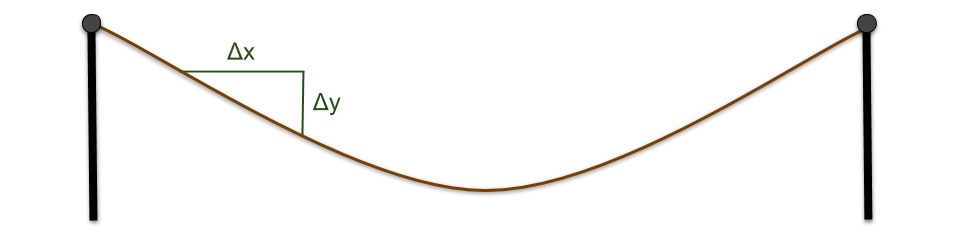
\includegraphics[width=.95\textwidth]{images/Dirichlet_Energy.png}
            \end{figure}
            Let $u\colon \Omega \subseteq \R^1 \to \R$ define a 1-dimensional membrane by considering the graph $y=u(x)$. The increase in length from stretching is
            \begin{align*}
                \sqrt{(\Delta x)^2+(\Delta y)^2}-\Delta x &= \left(\sqrt{1 + \left( \frac{\Delta     y}{\Delta x}\right)^2} - 1\right)\Delta x\\
                \stackrel{\Delta x \to dx}{\implies}&= \frac{1}{2}\left\|\frac{du}{dx}\right\|^2dx
            \end{align*}
        \end{frame}
        
        \begin{frame}{One Dimension}
            If we then measure stretching over the whole membrane $\Omega$, the energy of stretching is
            \[
            E=\int_\Omega \frac{1}{2} \left\|\frac{du}{dx}\right\|^2 dx.
            \]
            This is the energy is we want to minimize.
        \end{frame}
        
        \begin{frame}{The Dirichlet Energy}
            \begin{definition}
            Let $u\colon \Omega \subseteq \R^m \to \R$. The \emph{Dirichlet energy} is defined to be the functional
            \[
            \mathcal{E}\colon H^1(\Omega) \to \R
            \]
            given by
            \[
            \mathcal{E}[u]= \int_\Omega \frac{1}{2} \|\nabla u\|^2 = \int_\Omega \frac{1}{2} \langle \nabla u, \nabla u \rangle.
            \]  
            \end{definition}
        \end{frame}
        
        \begin{frame}{Harmonic Maps}
            \begin{definition}
            A \emph{harmonic map} is a map that is a stationary (critical) point of the Dirichlet energy functional.
            \end{definition}
            \pause
            \begin{question}
                What is a stationary point of a functional?
            \end{question}
            \pause
            \begin{answer}
                It is an analogous definition to stationary points for functions.
            \end{answer}
        \end{frame}
        
        \begin{frame}{Stationary Points of Functions}
            \begin{definition}
            Consider a function $f\colon \Omega \to \R$, then a \emph{stationary point} $(p_1,\dots,p_n)\in \Omega$ satisfies
            \[  
            \nabla_{\mathbf{e}_i} f(p_1,\dots,p_n) = 0 \quad \forall \mathbf{e}_i \in     \{\mathbf{e}_1,\dots,\mathbf{e}_n\},
            \]
            where $\nabla_{\mathbf{e}_i}$ is the directional derivative in direction $\mathbf{e}_i$.
            \end{definition}
        \end{frame}

        \begin{frame}{Stationary Points of Functionals}
            \begin{definition}
            Consider a functional $\mathcal{E}\colon H^1(\Omega) \to \R$, then a \emph{stationary point} $u\in H^1(\Omega)$ satisfies
            \[  
            \delta_v \mathcal{E}[u]=0\quad \forall v \in H^1_0(\Omega),
            \]
            where $\delta_v$ is a variation in ``direction" $v$.
            \end{definition}
        \end{frame}
        
        \begin{frame}{The Laplace Equation Example}
            Consider a variation in direction $v$ of the Dirichlet energy functional
            \begin{align*}
            \delta_v \mathcal{E}[u] \coloneqq \left.\frac{d}{d\epsilon} \mathcal{E}[u+\epsilon v]\right|_{\epsilon=0}&=0 \\
            \int_\Omega \nabla u \cdot \nabla v&= 0,
            \end{align*}
            which is the weak form of the Laplace equation,
            \[
            -\Delta u = 0.
            \]
            \pause
            \begin{remark}
            $\implies$ Solutions to the Laplace equation are harmonic maps.
            \end{remark}
        \end{frame}
        
        \begin{frame}{Generalizations}
            \begin{question}
            Can we generalize the Dirichlet energy and harmonic maps further?
            \end{question}
            \pause
            \begin{answer}
            Yes.  We can generalize the Dirichlet energy to maps between Riemannian manifolds.  Harmonic maps will still be critical points of this energy.
            \end{answer}
        \end{frame}
        
        \begin{frame}{On a Manifold}
            \begin{definition}
            A \emph{Riemannian manifold} $(M,g)$ is a smooth manifold $M$ with a position dependent inner product $g$.
            \end{definition}
            \pause
            \begin{itemize}
                \item $M$ is a \emph{smooth manifold} if
                \begin{itemize}
                \pause
                    \item $M$ locally looks like $\R^m$,
                    \item $M$ can be covered with coordinates in $\R^m$ smoothly.
                \end{itemize}
                \pause
                \item $M$ is \emph{Riemannian} if there is a smoothly varying inner product for tangent vectors on $M$.
            \end{itemize}
        \end{frame}
        
        \begin{frame}{On a Manifold}
            \begin{figure}
                \centering
                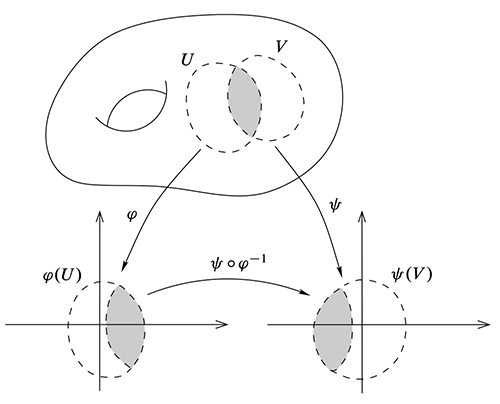
\includegraphics[width=.6\textwidth]{images/smooth_manifold.png}
                \caption{Giving $M$ smooth coordinates from $\R^m$.}
            \end{figure}
        \end{frame}
        
        \begin{frame}{Examples}
            \begin{example}
            $R^m$ itself is a Riemannian manifold with the Euclidean inner product.
            \end{example}
            \pause
            \begin{example}
            The \emph{round sphere} 
            \[
            S^m \coloneqq \{ (x_1,x_2,\dots,x_{m+1}) ~\vert x_1^2+x_2^2+\cdots+ x_{m+1}^2 = 1\}
            \]
            is a Riemannian manifold with the round (standard) metric inherited from the imbedding into $\R^{m+1}$.
            \end{example}
            \pause
            \begin{remark}
            Any smooth manifold $M$ can be made into a Remannian manifold.
            \end{remark}
        \end{frame}
        
        \begin{frame}{On a Manifold}
            \begin{definition}
            The Dirichlet energy for a map $u \colon (M,g) \to (N,h)$ is
            \begin{align*}
            \mathcal{E}[u] &= \underbrace{\int_{M} \frac{1}{2} \|du\|^2 d\textrm{Vol}_M}_{\textrm{coordinate free}} =  \underbrace{\int_{M} \frac{1}{2} g^{ij}h_{\alpha \beta} \frac{\partial u^\alpha}{\partial x^i}\frac{\partial u^\beta}{\partial x^j}d\textrm{Vol}_M}_{\textrm{local coordinates}}.
            \end{align*}
            A stationary point of this energy is a \emph{weakly harmonic map}.
            \end{definition}
            \begin{itemize}
                \item The matrix $\frac{\partial u^\alpha}{\partial x^i}$ is the Jacobian of the transformation.
                \item The Jacobian describes the stretching of space.
                \item Geodesics, minimal surfaces, and minimal submanifolds are all harmonic maps between manifolds.
            \end{itemize}
        \end{frame}
        
    \subsection{Gradient Flow}
    
        \begin{frame}{Finding Harmonic Maps}
            \begin{question}
                Is there any easier (possibly computational) way to find harmonic maps?
            \end{question}
            \pause
            \begin{answer}
                Yes.  We can flow to the stationary points of functionals via the gradient flow.
            \end{answer}
        \end{frame}
        
        \begin{frame}{Gradient Flow}
            In finite dimensions, (negative) gradient flow is given by following the path of steepest descent that limits to a stationary point.
            \begin{figure}[H]
                \centering
                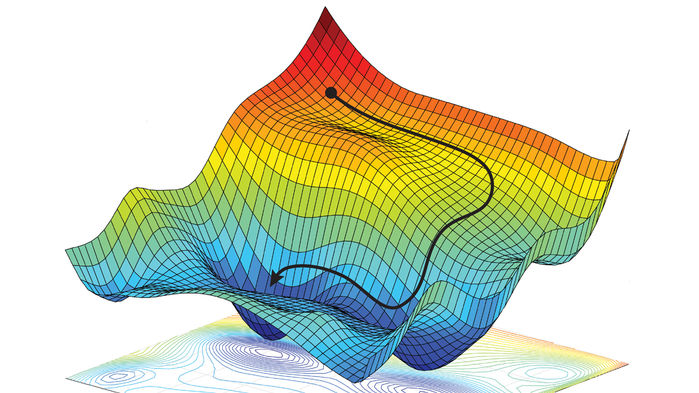
\includegraphics[width=.6\textwidth]{images/gradient_descent_surface.jpg}
                \caption{Thinking of our function as a surface, we let our curve follow the gradient field over time.}
                \label{fig:gradient_flow_surface}
            \end{figure}
        \end{frame}
        
        \begin{frame}{Finite Dimensional Gradient Flow}
        
        \begin{definition}
        The \emph{gradient flow} is a curve $\boldsymbol{\gamma}$ such that
        \[
        \frac{\partial \boldsymbol\gamma}{\partial t} = -\nabla f.
        \]
        Equivalently, the gradient flow in direction $\mathbf{e}_i$ is given by
            \[
            \left\langle \mathbf{e}_i ,\frac{\partial \position}{\partial t}\right\rangle = -\nabla_{\mathbf{e}_i} f \quad \forall \mathbf{e}_i \in \{\mathbf{e}_1,\dots,\mathbf{e}_n\}.
            \]
        \end{definition}
        \end{frame}
        
        \begin{frame}{Computational Method}
            \begin{figure}[H]
                \centering
                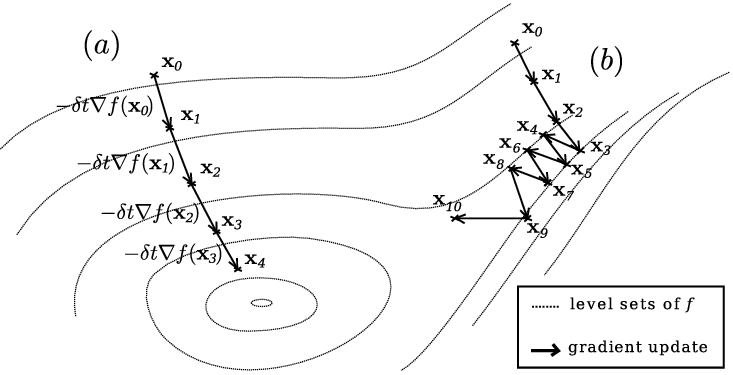
\includegraphics[width=.7\textwidth]{images/gradient-trajectory.png}
                \caption{A computational trajectory of the gradient flow.}
                \label{fig:gradient_trajectory}
            \end{figure}
        \end{frame}
        
        \begin{frame}{Gradient Flow in $H^1$}
        \begin{definition}
            The \emph{gradient flow} in $H^1(\Omega)$ in direction $v$ is
            \[
            \left\langle v,\frac{\partial u}{\partial t}\right\rangle_{L^2(\Omega)}=-\delta_v \mathcal{E}[u].
            \]
        \end{definition}
        \pause
        \begin{remark}
            This will give us a weak form of a PDE.
        \end{remark}
        \end{frame}
        
        \begin{frame}{The Heat Equation Example}
            We can then take the gradient flow in direction $v$ by
            \begin{align*}
            \left\langle v,\frac{\partial u}{\partial t}\right\rangle_{L^2(\Omega)}&=-\delta_v \mathcal{E}[u]\\ 
            &~\Big\downarrow\\
            \int_\Omega v\frac{\partial u}{\partial t} &= -\int_\Omega \nabla u \cdot \nabla v 
            \end{align*}
            Which is the weak form of the source free Heat equation
            \[
            \frac{\partial u}{\partial t} - \Delta u = 0.
            \]
        \end{frame}
        
        \begin{frame}{Answering the Question}
            \begin{question}
            What is a stationary point for the functional $\mathcal{E}$?
            \end{question}
            \pause
            \begin{answer}
            The limit as $t\to \infty$ of our gradient flow.
            \end{answer}
        \end{frame}
        
        \begin{frame}{Putting it All Together}
            With this framework, we can answer the motivating problem of finding harmonic maps. 
            \pause            
            \begin{problem}[Geodesics]
            Consider a rope $\gamma$ with endpoints $\gamma(0)=p$ and $\gamma(1)=q$ fixed on a surface $M$.  What is the shortest configuration for this rope?
            \end{problem}
            \pause
            \begin{answer}
            The minimal $\gamma$ is a harmonic map.  We can start with any rope, and we can pull the rope tight from each side by performing gradient flow.  Once the rope is pulled tight, we are left with a geodesic.
            \end{answer}
        \end{frame}
        
        \begin{frame}{Further Questions}
            \begin{itemize}
                \item How do we handle cases with external forces?
                \item What if we put further constraints on our system?
                \item How do we know we've achieved a minimizer?
            \end{itemize}
        \end{frame}
        
        
\end{document}